% This is samplepaper.tex, a sample chapter demonstrating the
% LLNCS macro package for Springer Computer Science proceedings;
% Version 2.21 of 2022/01/12
%
\documentclass[runningheads]{llncs}
%
\usepackage[T1]{fontenc}
% T1 fonts will be used to generate the final print and online PDFs,
% so please use T1 fonts in your manuscript whenever possible.
% Other font encondings may result in incorrect characters.
%
\usepackage{graphicx}
% Used for displaying a sample figure. If possible, figure files should
% be included in EPS format.
%
% If you use the hyperref package, please uncomment the following two lines
% to display URLs in blue roman font according to Springer's eBook style:
%\usepackage{color}
%\renewcommand\UrlFont{\color{blue}\rmfamily}
%
% \usepackage{wrapfig}
%
\begin{document}
%
\graphicspath{ {./figs/} }
%
\title{An Ontology-based Knowledge Management Model on Information Governance}
%
%\titlerunning{Abbreviated paper title}
% If the paper title is too long for the running head, you can set
% an abbreviated paper title here
%
\author{First Author\inst{1}\orcidID{0000-1111-2222-3333}}
%
\authorrunning{C. Mega et al.}
% First names are abbreviated in the running head.
% If there are more than two authors, 'et al.' is used.
%
\institute{University on Stuttgart, Stuttgart, Germany
\email{cataldo.mega@ipvs.uni-stuttgart.de}\\
\url{https://www.ipvs.uni-stuttgart.de/departments/as/}}
%
\titlerunning {IGO an Ontology on Information Governance} 
\maketitle              % typeset the header of the contribution
%
\begin{abstract}
Information is a strategic asset to enterprises and subject to Information Governance (IG) as mandated by corporate and regulatory compliance. Overall governance goals are the management and control of business relevant data such to minimize legal risks and reduce operational cost. Recent surveys show that around 40\% of companies have insufficient IG practices in place and are exposed to higher compliance risks. Where there exists an IG Strategy, its implementation is typically homegrown, difficult to integrate and error prone. Our investigation shows that a major impediment to implementation and interoperability is the lack of a common language. One that defines what information governance consists of in technical and operational terms. In addition, the many existing frameworks in this domain make the exploitation of the available knowledge and definition of standardized IG specific services very difficult, often leading to costly one-off implementations. A solution to this problem is the availability of a common and unambiguous domain vocabulary as a pre-requisite to a commonly accepted ontology on information governance. This paper suggests an ontology-based framework (IGONTO) that supports the creation of a knowledge store that facilitates access of domain knowledge through semantic search.

\keywords{Enterprise Information Management \and Information Governance \and Ontology \and Knowledge Graph \and Cloud-Services}
\end{abstract}
%
%
%
\section{Introduction}
Our work is premised on the basis that domain knowledge, expertise and technology on information governance solutions exist in abundance but scattered around and difficult to get hold on. In order to aid companies to find the blueprint of an IG solution that suites their needs the existing knowledge must be collected, synthesized, and offered as a service, accessible to humans and machines in an easy and cost-effective way. We believe this is best done through the use of an ontology-based model on information governance. 

Our suggestion is to create an information governance graph based on an ontology constructed with a rich semantic model. We envision a graph store containing generalized information of governance concepts, components modelled from functional, non-functional and operational requirements together with a list of design artefacts that expose key IG capabilities and functions.

 \begin{figure} [h]
 %\centering
%\includegraphics[page=1,trim=0 1cm 0 0,clip, width=\textwidth]{IGSModelsMedium.pdf}
\includegraphics[page=1,trim=0 1cm 0 0,clip, width=345pt, height=130pt]{IGSModelsMedium.pdf}
\caption{Process pipeline from knowledge acquisition to service implementation.} \label{fig1}
\vspace{-10pt}
\end{figure}

Figure~\ref{fig1}. outlines this approach showing the processing pipeline. Starting from left to right you see: Step 1 acquisition phase, where is the knowledge, vocabularies terms, guidelines, standards, and best practices are acquired from the IG domain. Step 2 processing phase, the information processed in a way to a taxonomy of related concepts, associated rule sets and their descriptions.  

Step 3 access phase, this is where we create the ontology (semantic schema) and load instance data (individuals) in to the knowledge graph. Step 4 delivery phase, at this point users are able to retrieve design models and service templates as constituent parts of an IG solution blueprint and respective build plans. 

The result is IGONTO, a framework consisting of a harmonized information governance vocabulary, a semantic schema (IGO), a knowledge graph (IGG) and a repository (IGREPO) of design artefacts that aid the development of an IG solutions architecture. It provides a way for interested parties to use the framework as a knowledge system for generating state-of-the-art design models and building blocks such for being able to compose the envisioned IG solution. 

The remainder of this paper details our approach and is structured as follows: Section 2 introduces briefly some of the key aspects on governance and more specifically information governance. It then describes the business problem and explains it with a concrete use case scenario. Section 3 is a summary of our contributions. Section 4 is about the governance domain analysis which we conducted and what we learned. Section 5 uses the results of section 4 and discusses the IG taxonomy and ontology we created illustrating the concept graphs obtained. Section 6 presents related work and section 7 our concluding remarks.

\subsection{Governance Domains}
Governance at its core is about corporate and regulatory compliance based on trust fueled by continuous IG practice, monitoring its effectiveness and control. It consists of responsibilities and commitments implemented by processes that ensure proper data access, implement guidelines and legal requirements. As such, corporate governance (CG) in an enterprise ensures that valuable information adhere with proper quality standards related to data authenticity, integrity and reliability in compliance with regulations. In summary, today’s enterprises are governed by a framework of principles, values, policies and processes intended to help organizational units to move towards shared corporate compliance goals.

The principal design criteria of governance have a focus on enabling information quality strategies and to classify process capabilities against an Information Governance Maturity Model (Pierce, 2007).
 This means, at its core governance models cover three major responsibility domains: i) Corporate Governance (CG), ii) Information Governance (IG) and iii) IT Governance (ITG) which we outlined in Figure 2. Each domain addresses different governance areas using frameworks suitable for one or the other, emphasizing more the organizational or implementation aspects. 
 
The left-hand side of Figure~\ref{fig2}. shows Information Governance and its relationships to the Information Management, Content Management, Records Management and Asset Management categories.

 \begin{figure*}
 %\centering
%\includegraphics[page=2,trim=0 2cm 0 0,clip, width=400pt, hight=80pt]{figs/IGSModelsMedium.pdf}
\includegraphics[width=\linewidth]{IGSModelsMedium.pdf}
\caption{Corporate governance domains.} \label{fig2}
\end{figure*}

These categories represent the context in which data is processed. Their functional areas are driven by information governance life-cycles that perform activities to apply compliance policies and enforce rules on how to handle corporate data and information. Similarly, IT Governance, as shown on the right-hand side, relates to IT operations rules applied to infrastructure, processes, performance, risk, and input \& output management enforcing corporate compliance goals ensuring accountability, transparency, responsibilities and minimizing possible risks.

The focus of the remainder of this paper is on information governance (IG) with occasional references to the other domains, where required. 

\subsection{Problem Description} 
From experience we learned that the success of information governance and regulatory compliance in companies depends on a common understanding conveyed through an unambiguous language. Thus, such a language is an important pre-requisite to design, implementation and deployment of the required data governance services and their controls. On the other hand, the actual requirements of an information governance strategy depend on the type of data processed and the business context they belong to. 

For organizations this implies a responsibility to implement information governance practices that enforce proper data usage in their specific production environment throughout the entire information life-cycle. The problem though is that even after knowing ‘what is’ required, many companies face challenges with the architecture design of their individual IG solution because of the many technology and product options available on the market. These circumstances translate into a lengthy and formal process of announcing new information governance projects through a Request for Proposal (RFP) where in response, qualified contractors submit bids to undertake the project. Typically, the RFP document contains detailed information about the project, requirements, and evaluation criteria.

The good news is that typical information governance solutions follow on an architecture blueprint that is composed of well-known software design patterns, available domain knowledge and experience. Luckily enough, software instances of IG building blocks are available in a variety of IG product offerings from open source and different vendors. Therefore, our conclusion is that by exploiting the available knowledge it is possible to generate the required information of components and design artefacts for allowing companies to compose IG solutions instead of custom developing new ones. 

Exactly this is the goal of our IGONTO approach as depicted in Figure~\ref{fig1}. This motivates the use of ontologies and knowledge graphs to store domain knowledge and to make it available through semantic search with the benefit that on a global and open information market this knowledge is made accessible programmatically facilitating the sharing of data and services. We think ontologies can expedite access and retrieval of IG service building blocks where the requirements defined in concept entities are matched by the capabilities of design entities and corresponding implementation components and their building blocks. 
%%
\subsection{Usage Scenario}
Let us look at a real-world IG use case scenario explain our approach. 
Assume a company having the following business requisites:

\begin{enumerate}
    \item Business Data Type: Personal Identifiable Information (PII), customer contractual data and related contextual information; 
    \item Business presence in countries: US, EU; 
    \item Jurisdictions of interest: US, EU; 
    \item Applicable regulations: US Privacy Act, EU GDPR; 
Regulatory compliance with these business requisites translates into the following functional and non-functional requirements: 
    \item R1: Contractual and legal obligations require the company to collect and classify person and business data as well as related contextual information from pre-contract and contract activities. 
    \item R2: Data must be persisted reliably, after verifying its authenticity and integrity. 
    \item R3: Data is stored for as long as required by business, legislations and regulations.
    \item R4: Access to stored data is controlled by security and privacy policies. 
    \item R5: Data is deleted or barred from access upon lapse of a storage period prescribed by business or legal instruments. 
\end{enumerate}

Figure~\ref{fig3} outlines the use case scenario in form of a semantic graph subdivided into four functional domains. Capitalized terms printed in bold represent key IG concepts. Dashed boxes are used to emphasize their affiliation domain: Corporate Governance, Information Governance, Implementation and Platform domains.

The upper left dashed box outlines graphically the business requisites. This reads like this: a Company has a business presence in the Countries: EU and US. Their Jurisdictions are regulated by the US Privacy Act (GSA, 2022)and the EU GDPR Regulations (EU, 2018). Thus, this Company by law has to implement an IG solution consisting of a number of governance principles that address: Security, Privacy and Integrity concerns.

\begin{figure} [h]
 \centering
\includegraphics[page=3,width=.8\textwidth]{IGSModelsLarge.pdf}
\caption{IG-Scenario concept classes and their relationships by domain.} \label{fig3}
\end{figure} \vspace{-10pt}

This means, each category shown consists of a number of requirements and obligations that have to be satisfied, like: 
\begin{enumerate}
    \item R6: verify Data Authenticity, 
    \item R7: ensure Data Integrity and 
    \item R8: provide system and Service Reliability. 
\end{enumerate}

From an implementation stand point these requirements translate into the following guidelines:
\begin{enumerate}
    \item GL1: “…in order to reach a governance maturity level 4 an organization must implement a Metadata Definition Process that is an integral part of the implemented Records Management Practice …see Figure~\ref{fig3}.”  In addition, the US Privacy Act mandates that:
    \item GL2: “… Data and software integrity failures must be monitored, assessed, monitored and mitigated,…”. 
\end{enumerate}

The dashed box labeled Implementation in Figure~\ref{fig3}. lists the concept classes mentioned in the guidelines: Data, Metadata, and Records Management Practice, they all relate to Processes that satisfy the associated requirements through inferred system components. The line of thought at concept level follows this logic: 

The Metadata Definition Process is responsible for creating necessary governance metadata that describe how data is processed and stored based on applicable corporate and regulatory Policies. 

Following well known domain best practices, implementing such an IG-Program employs the availability of Repositories where Data and related Metadata is securely stored. 
In this context, data is subject to different Lifecycles and controlled by a Records Management System. 

Records Classification processes classify the data in to categories and assign specific Policies used to control Access, Retention and Disposition by means of appropriate Rules. Repositories typically use Databases, Full Text Indexes and Storage Systems representing IT Resources that are provisioned by Platform Services. 

 In a subsequent refinement step the concepts of Repository and Database are then mapped on to the implementation concept/classes following the relationships links from class to class:
 \begin{enumerate}
     \item Repository -> Content Repository-> Content Services -> Alfresco Content Services 
     \item Repository -> Metadata Repository -> Database Service -> Database -> PostgreSQL. 
 \end{enumerate}
As shown in the graph on the bottom of Figure~\ref{fig3}.

With this approach, it is possible to identify the right components to build an IG solution following a well-known solutions architecture like the one shown in Figure~\ref{fig4}. 

The blueprint in Figure~\ref{fig4}. outlines on the left, the data sources of an enterprise from where data is collected, pre-processed and classified. 

Classified data is then loaded in an enterprise information systems (EIS) and put under control of an information lifecycle designed to handle data of a specific type. Lifecycle processes create required governance metadata before both data and metadata are persisted on storage systems managed by a Content Management system. In a post-processing environment, shown on the right side of Figure~\ref{fig4}, you see Enterprise Records, Case Management, eDiscovery and Content Analytics components.  These services produce the required governance information such to satisfy audit trails, statistics and reporting needs. The comparison of Figure~\ref{fig3} with Figure~\ref{fig4} shows the mapping between concept classes, design components and services. 

The gist of what this use case is trying to convey is that with the given business requisites and based on the defined semantic model, it is possible to generate a list of concept artefacts having the capabilities and characteristics for satisfying the implied functional, non-functional and operational requirements with the aid of a knowledge store. 

In summary we observe that a successful IG-Program implementation depends directly on an efficient enterprise information system where governance is achieved through adjustments of the information management practice with ongoing monitoring, assessment and reporting. 
%
\begin{figure} [h]
 \centering
\includegraphics[page=4, width=.8\textwidth]{figs/IGSModelsLarge.pdf}
\vspace{-10pt}
\caption{IG solution blueprint and its major components.} \label{fig4}
\end{figure} %\vspace{-10pt}
%
%%
\section{IG Domain Analysis}
This section briefly introduces the domain sources we evaluated in our effort to identify valuable IG knowledge, concept classes and their meaning. 
Table~\ref{tab1} shows a representative list of practitioner organizations and public agencies, their frameworks and scope. Common to the taxonomy employed by each framework is a 3-level category structure. Column 2 in Table~\ref{tab1} outlines the overall scope of each governance frameworks and its functional areas: General Governance Principles (IGMM), IG Reference Model (IGRM), Electronic Discovery Reference Model (EDRM), IT Governance Suite, Digital Asset Management, and Data Management Framework.

\begin{table}
\caption{IG Frameworks.}\label{tab1}
\begin{tabular}[0.5\textwidth,center]{|l|l|}
%\hline
\multicolumn{1}{c}{\textbf{Organization}} & \multicolumn{1}{c}{\textbf{Framework/Scope}}\\ \hline
ARMA & IGMM - IG Maturity Model – Principles \\  \hline
CGOC/EDRM (EDM C. , 2021) & IG Reference Model\\
     & Electronic Discovery Reference Model\\ \hline
ISACA & COBIT - IT Governance Suite\\ \hline
DAM & Digital Asset Management\\ \hline
DAMA  & Data Management Framework\\ \hline
NARA/CRL(US) & National Archives\\
(NARA, 2006) & Records Administration, \\
             & Records Management, \\
             & Center of Research Libraries \\ \hline
\end{tabular}
\end{table} 
\,  % cuts the line space in half 

The main categories used across the frameworks are: Accountability, Transparency, Integrity, Protection, Compliance, Availability, Retention and Disposition. These categories apply for both the organizational or functional areas. Each category has a number of context specific capabilities and/or requirements assigned. They represent concept/class attributes or relationship properties. 

The frameworks also introduced a scalar metric called governance maturity level (GML), with a value range from 0 to 5 (i.e. ad hoc to a fully functional IG-Program implementation). GML is computed from a specific subset of capabilities and requirements that must be satisfied by context and category. 

The last row of Table~\ref{tab1} lists (NARA, 2006) and CRL both represent government agencies. They share a framework with a focus on the records management lifecycles and aspects to manage and operate Records and Content Management System and Digital Archives. The given guidelines draw requirements from relevant standards like NIST.IR.8286C (Quinn S, Barrett, \& Witte G, 2022) (ISO-15489, 2016). The international ISO standards evaluated, with their applicable domain are listed in Table~\ref{tab2}. 

\begin{table} [ht]
\caption{ISO Standards.}\label{tab2}
\begin{tabular}{|l|l|}
%\hline
\multicolumn{1}{c}{\textbf{Organization}} & \multicolumn{1}{c}{\textbf{Standards}} \\ \hline
(ISO-14271,2017) & {Open Archive Information System} \\ \hline
(ISO-15489, 2016) & { Records Management: Concepts and Principles.}\\ \hline
(ISO-16363)  & {Audit and certification.} \\ \hline
(ISO-27000) & ISO family of standards related to \\
    & Information Security Management Systems (ISMS) \\ 
    & including Information security, cyber-security, \\
    & privacy protection and \\
    & risk management guidelines.\\ \hline
\end{tabular}
\end{table} 
\,  % cuts the line space in half 

Table~\ref{tab3} shows 3 privacy regulations in force in the US, EU and DE jurisdictions. We included them as they represent the security and privacy categories. The 2 major principles of governance these days.

\begin{table}
\caption{Regulator \& Regulations}\label{tab3}
\begin{tabular}{|l|l|}
%\hline
\multicolumn{1}{c}{\textbf{Regulator}} & \multicolumn{1}{c}{\textbf{Regulations}}\\ \hline
US GSA & US Government Services Agency \\
       & Directives: Privacy Act (GSA, 2022)\\ \hline
Europe & General Data Protection Regulation (EU, 2018)\\ \hline
Germany  & DE Datenschutz-Grundverordnung \\ \hline
\end{tabular}
\end{table}   
\,  % cuts the line space in half 

Interesting to note: Ensuring compliance with these regulations already employs a complex implementation model involving elements of core Enterprise Information Systems (EIS) concepts like the ones we introduced and discussed in the use case scenario of section 2.3 and outlined in form of a semantic graph in Figure~\ref{fig3}.

Moving from business to implementation concepts we searched for standards related to enterprise information management (EIM) systems and looked at their design models. The 3 Standards of interest are listed in Table~\ref{tab4}. These are 2 OASIS standards: a) CMIS, the “Content Management Interoperability Services” standard, b) TOSCA the “Topology and Orchestration of Specification for Cloud Applications” and c) the “Trustworthy Digital Repositories” specification which was standardized in ISO-14271.

\begin{table}
\caption{OASIS CMIS, TOSCA and ISO-14721 OAIS }\label{tab4}
\begin{tabular}{|l|l|}
%\hline
\multicolumn{1}{c}{\textbf{Organization}} & \multicolumn{1}{c}{\textbf{Standards}}\\ \hline
OASIS & CMIS Content Management Interoperability Services (CMIS, 2015) \\
      & TOSCA - Topology and Orchestration of \\
      & Specification for Cloud Applications (TOSCA, 2020)\\ \hline
NASA / ISO & Trustworthy Digital Repositories; \\ 
        & (ISO-14271, 2017) / (CCSDS 650.0-B-1)\\ \hline
\end{tabular}
\end{table}  
\,  % cuts the line space in half 

All three standards are well suited for our approach as they provide the required links between the business/governance and systems/design concepts. 
In order to create a complementary IG graph store (IGG), we collected concept/class instances (individuals) from open source and commercial services offering and classified them by functional area and capabilities. Table~\ref{tab5} shows the group of vendors and lists their product and platform services related to key IG classes and functional components.
\begin{table} [h!] 
\caption{Vendors and their service offerings}\label{tab5}
\begin{tabular}{|l|l|}
%\hline 
 \multicolumn{1}{c} {\textbf{Vendor}} & \multicolumn{1}{c} {\textbf{Products}}\\ \hline
Alfresco & Alfresco Digital Business Platform: \\
         & Content, Process \\
         & Governance Services (ACS, APS, AGS) (Alfresco, 2021) \\ \hline
Open Text & OpenText / Documentum (OpenText, 2022)\\ \hline
IBM  &  Content Manager, FileNet, OnDemand and Co-Products (IBM, 2022)\\\hline
Microsoft  &  Office 365 and Co-Products (ref) \\ \hline
Oracle  &  Oracle Cloud Services (ref)\\ \hline
Google  & Google Cloud Services (ref)\\ \hline
Amazon  &  Amazon Cloud Services (ref)\\ \hline
Open Source  &   CNCF,2022 (Docker, Kubernetes), others\\\hline
\end{tabular}
\end{table} 
\,  % cuts the line space in half 

For our ontology, we considered subsets of the above presented vocabulary terms and concepts. All those related to services design, their implementation and operational aspects. Additionally, the ISO standards documentation provided relevant contextual information which we used to harmonize the chosen terms before including them in the IGO semantic schema. 
The vendor sources also provided domain knowledge on information management and governance through their cross-cloud platform product offerings. 

A common understanding in the IG domain is that information governance fundamentally involves services, applications and infrastructure capable of maintaining governance information at a high-quality level such to support business decisions in an effective and timely fashion. 
Overall, through our research we found that standards and regulations specify what has to be done and what must be avoided when implementing an IG program. Whereas frameworks emphasize more on guidelines and how corporate and regulatory compliance can be achieved, such to reach a specific governance maturity level. 

Implementing an IG program requires state-of the art technology and methods that promote flexible and efficient operations favoring the creation of business value and reduce business, compliance and regulatory risks. (ISO-14271, 2017), (NARA, 2006), NIST (2022)
Companies in their actual implementation efforts can take advantage from information and artefacts delivered by open source communities, payable services and online platforms complementing their in-house development without going through a lengthy RFP process. 
%%
\subsection{Contributions}

Our contribution can be summarized as follows: we created an IG taxonomy, used it to design an ontology (IGO) based on harmonized concept terms and formalized relationships. Built an IG Graph (IGG) loaded with instances (individuals) annotated with domain knowledge on best practices, guidelines and service descriptions and made this knowledge accessible through semantic queries. To complement the ontology and the IG graph we created also   

IGREPO a repository of best practices documentation, guideline documents and prototype implementations of service templates written in their domain specific language (DSL) i.e. TOSCA and YAML.

%% -------------------------------------------------------------------------------------------

\section{IG Knowledge Models}
This section details our ontology (IGO). Due to the large number of concept/classes we first reorganized the governance classification scheme into 6 top level categories and 26 sub-categories. For each top-level category we created an ontology. These are: Organization (ORG), Information (INF), System (SYS), Component (CPT), Lifecycle (LCS) and Platform (PLT). 

We then harmonized the vocabulary terms by sub-category and aligned them according to their relevance and the functional area they belong to. Each sub-category consists of a number of requirements, capabilities, recommendations and domain constraints. Together they form the overall IGO concept model. 

The foundational ontology is Organization. It is composed of the child level categories: Agent, Goal, Objective, Quality, Compliance and Responsibility. They form the high-level concepts forming a semantic graph that represent an Organization and its associated concept classes in our context.  Each class has a description, relations (object properties), attributes (data properties), comments and annotations, all of which synthesized from domain knowledge, best practices, and guidelines. This knowledge is formalized and used to create the semantic schema and the IG graph store.

Formal description logic is used to ensure that concept descriptions utilize unambiguous semantics and well-formed rule sets readable by both machines and humans. Inference is achieved following the class relationships built-in the semantic graph representing. 

The following 6 sub-sections introduce at the high-level the 6 ontologies by category. One level below you see instances of Organizational Unit and its instances: Business, Legal, Records Management, Architecture and IT, the typical Departments of Enterprises.

%%
\subsection{Organization Model}

Model Description: Figure:\ref{fig5} shows the Organization semantic graph with top-level concepts: Organization, Organizational Unit, Enterprise, Department on one side and Governance, Governing Body and Steering Committee on the other side. Departments produce Data and Metadata through their services and processes. Steering Committees define long term goals and short-term objectives like Quality and Compliance with Regulations and legal obligations.  

 \begin{figure}[h] 
 \centering
\includegraphics[page=5,trim=0 0.5cm 0 1cm,clip, width=\textwidth]{figs/IGSModelsMedium.pdf}
\caption{Organization Model.} \label{fig5}
\end{figure} 

The lower right corner in Figure:\ref{fig5} lists Employees who vest Roles that are associated with Responsibilities and employed duties like CGCO* , CISO* , and DPO*.
%-------------------------------
\subsection{Information Model}

Model Description: The Information ontology (INF) is constructed around the key concept of Data. It lists Content, Metadata and Asset as derived classes representing digital objects of any type and format. In this model, an Asset represents a data container that links (aggregation relationship) together digital content, its metadata and associated contextual information. At concept level Information is shown as being derived from Metadata that in turn is itself derived from data. 

 \begin{figure}[h] 
 \centering
\includegraphics[page=6,trim=0 1cm 0 0.5cm,clip, width=\textwidth]{figs/IGSModelsMedium.pdf}
%\includegraphics[page=6,keepaspectratio, width=7.5cm,height=5cm]{figs/IGSModelsMedium.pdf} 
\caption{Information Model.} \label{fig6}
\end{figure}

The right side of Figure ~\ref{fig6} shows the governance metadata model starting with the key concept of Record and its relation to Data. This means, a Record represents a set of governance metadata consisting of classification information used to define process control information for Data security, privacy, retention and disposition. Such processes are controlled by Policy instances containing Rules specific to the Data category and Lifecycle phase in which the Data is being processed. 

From a governance standpoint, the concept of a Policy is the control mechanism assigned to data after its classification, according to applicable taxonomies. 
By definition, a Policy class aggregates Goal, Rule and Metric and is used by an information governance Lifecycle workflow that enforces rules, collect metrics and drive processes for satisfying set corporate goals. Goals, Rules and Metrics depended on whether it refers to Content, Metadata, Asset, Records or collateral Information. 

Assets have value, cost and risk and controlled by governance policies that employ the rules used to steer the organization towards the wanted information management and governance course.  
Typically, access to persisted data is secured by a security policy in a way that data objects are assigned access control permissions and roles are given a set of privileges i.e. rights. 

To a Subject requesting to retrieve a specific data object, access is granted if the Subject vests a Role, where the roles privileges do match the permission assigned to the Data Object. 
Value, cost and risk of Data depend on time; therefore, the applied policies must change over time and thus require an ongoing process that adjusts policy rules accordingly. 

Typical data storage rules are R1) Data with no value V (t) =0 and must be deleted to reduce cost; R2) Data with high value must be kept forever, but to reduce cost it has to be moved onto less expensive storage. R3) PII Data must be stored and handled according to regulations by jurisdiction.
%-------------------------------
\subsection{System Model}

Model Description: The Systems semantic model entails the core concepts of the implementation domain (see the graph in Figure~\ref{fig3}). 

The vocabulary terms used in this model, reflect key concepts related to the architecture and design of an IG solution that are based on requirements related to the IG program and its implementations. Top-level classes are Architecture, Design, Model and model instances, including: Data- and Information Model down to the Deployment and Execution Model.

\begin{figure}[h] 
 \centering
%\includegraphics[page=7,keepaspectratio, width=10cm,height=7cm]{figs/IGSModelsMedium.pdf} 
\includegraphics[page=7,trim=0 0.5cm 0 0.5cm,clip, width=\textwidth]{figs/IGSModelsMedium.pdf}
\caption{System Model.} \label{fig7}
\end{figure}

The Architecture and Design terms listed in Figure~\ref{fig8} represent the system characteristics and design models of an Enterprise Information System (EIS). The semantic schema outlined shows the relationships between Architecture and other systems components. It explains what they do and how to use them. 


The lower part of Figure~\ref{fig8} shows the internal structure of an EIS system, consisting of a number of service components: Content, Information Retrieval, Analytics services and their relations to Data, Metadata and the Repository to which they belong. 
A Repository in turn utilizes a Catalog and a Full Text Index as its source of information. Last in this hierarchy is the Execution Environment and the Platform. Both are concepts native to the Infrastructure as a Service (SaaS) domain that describe how infrastructure resources of the type Compute, Network and Storage are provisioned or de-provisioned.
%-------------------------------
\subsection{Component Model}

Model Description: The Component ontology shown in Figure~\ref{fig7} lists concepts corresponding to the major functional areas covered by an IG framework, being: Administration, Maintenance, Management, Security, Privacy, Function, and Records. Function in this context is both a concept and a category referring to: Collect, Store, Access, Index, and Classify components representing software that exposes those capabilities. 

\begin{figure}[h] 
 \centering
\includegraphics[page=8,trim=0 1cm 0 1cm,clip, width=\textwidth]{figs/IGSModelsMedium.pdf}
%\includegraphics[page=8,keepaspectratio, width=7.5cm,height=5cm]{figs/IGSModelsMedium.pdf} 
\caption{Component Model.} \label{fig8}
\end{figure}

Through the IGONTO framework, these concept/classes are mapped to pre-existing software services provided online and modelled as service junction-points that use standard communication protocols to form cross-platform data processing pipelines.
%-------------------------------
\subsection{Lifecycle Model}

\textit{Model Description:} The governance Lifecycle model aggregates concepts related to services and processes bound to workflows that steer the data processing chain. 
\begin{figure} {l}{0.6\textwidth}
 %\centering
\includegraphics[page=9, scale=0.5]{figs/IGSModelsMedium.pdf} 
%\includegraphics[page=9,keepaspectratio, width=7.5cm,height=5cm]{figs/IGSModelsMedium.pdf} 
\caption{Lifecycle Model.} \label{fig9}
\end{figure}
They enforce corporate governance policies using appropriate methods along the process pipeline (see Figure~\ref{fig1}) and collect records metadata state. The lifecycles describe aspects on how data is moved from one phase to another based on state change that trigger data flow direction turns.The lifecycle logic monitors state information.  

Figure~\ref{fig9} lists Processes at the lowest level. They monitor the handling of data in their business production environment and produce complementary tracking information to ensure and safeguard the Chain of Custody. Process transparency is achieved through collection of audit data.

%%----------------------------
\subsection{Platform Model}

Model Description: The Platform ontology (PLT) models the platform level. It defines concepts that describe the execution environment, in which a system, its component and required infrastructure resources are deployed and orchestrated. 

\begin{figure} {l}{0.7\textwidth}
 %\centering
\includegraphics[page=10,trim=0 1cm 0 1cm,clip, width=0.6\textwidth]{figs/IGSModelsMedium.pdf}
%\includegraphics[page=10,keepaspectratio, width=7.5cm,height=5cm]{figs/IGSModelsMedium.pdf} 
\caption{Platform Model.} \label{fig10}
\end{figure}

For this ontology we collected descriptions of pre-defined (TOSCA, 2020) service templates, their capabilities and relationships. Each service template describes at concept level the required infrastructure resources, the runtime environment, the build plans and the orchestration logic. Usage notes complements the information with the instruction of how to map a TOSCA services template to a vendor specific service instance and the underlying deployment platform all stored in the artefact repository.
%%
\section{Related Work}
(DeStefano, Tao, \& Gai, 2016) inspired this work using a similar approach but used it for a different data governance problem. (Pierce, 2007)outlines the principal designing criteria on data governance. (Casonato, 2011) elaborates on the relationship between Enterprise Information Management and Information Governance showing that IG is an extension of EIM. (Niemi, 2013) lays out the design of a Data Governance Framework. 

(Leibtag, 2014) explains the necessity of governance in enterprises. (Salman Kanbar, 2015) explores data governance in real world use case scenarios. (Proença, et al., 2018)re-elaborates on a maturity model for information governance IGMM). (Cheng, Li, Gao, \& Liu, 2017) looks at the governance maturity model and its implementation investigating the impact of storing and managing data in the context of cloud. (Yamada \& Peran, 2017) suggests a governance framework for enterprise analytics and data. (Al-Ruithe, Benkhelifa, \& Hameed, 2018) compares data governance on cloud versus non-cloud environments. (Abraham, Brocke, \& Schneider, 2019) reviews data governance conceptual frameworks suggesting a research agenda on white spaces in the IG research areas. 
(Yebenes Serrano \& Zorrilla, 2021) looked at a data governance framework for Industry 4.0. (Behringer \& Hizli, 2021) draws a global picture showing the current state-of-the-art on data governance. (Mahanti, 2021) introduces the topics of Data, Data Governance, and Data Management. Many ISO international standards relate to information governance like: (ISO-14271, 2017), (ISO-15489, 2016), and the ISO family of standards (ISO-27000). 

We re-used the vocabulary terms shared with the IG frameworks. Little work was found related on how to implement an IG framework from concept to an actual implementation on cloud platforms using pre-defined services. Nor have we found the definition of a semantic schema on information governance (ontology) or an associated IG graph built from existing domain knowledge. (Mubarkoot \& Altmann, 2021) published some on software compliance and  (TOSCA, 2020) in the context of information governance. We found also valuable concept work in W3C FIBO ontology from (EDM \& Council, 2020). 

We used all this related work as sources to extract relevant IG information, best practices and publicly available solution artefacts which we used to prototype the approach.

\section{Conclusions and Outlook}
This paper describes our ontology-based knowledge management model on Information Governance and presented the IGONTO framework. Major effort in our work was to collect domain knowledge from available IG frameworks and evaluated their taxonomies, vocabularies, glossaries and best practices. We re-engineered the taxonomy, enhanced the terms that represent core IG concepts, defined the semantic schema (IGO) and created a knowledge graph (IGG) accessible by human and machine-driven reasoning. In order to store solutions components, we added also an artefacts repository (IGREPO). 

Our work provides a way for interested parties, to use our framework as a system that makes domain knowledge and experience explicit and accessible through semantic queries. Result sets produced consist of generalized service concepts including descriptions of their functional, non-functional and operational capabilities and a list of IG program requirements they satisfy. We think of it as an accelerator for building information governance solutions composed of pre-defined IG services artefacts offered on clouds discovered through an IG-graph store.
As an outlook on future work, we are currently refining the IGO prototype and working on a IG-DSL to extend TOSCA such to provide a stronger bridge between concept and implementation.  

\subsubsection{Acknowledgements} TBD.
%
% ---- Bibliography ----
%
% BibTeX users should specify bibliography style 'splncs04'.
% References will then be sorted and formatted in the correct style.
%
% \bibliographystyle{splncs04}
% \bibliography{mybibliography}
%
\begin{thebibliography}{8}
\bibitem{ref_1} Abraham, R., Brocke, J. v., \& Schneider, J. (2019, July). Data Governance: A conceptual framework, structured review, and research agenda. International Journal of Information Management, 49. \doi{10.1016/j.ijinfomgt.2019.07.008}
\bibitem{ref_2} Alfresco. (2021). Alfresco Content Services. Retrieved from Alfresco Content Services: \url{https://www.alfresco.com/platform}
\bibitem{ref_3} Al-Ruithe, M., Benkhelifa, E., \& Hameed, K. (2018, January). Data Governance Taxonomy: Cloud versus Non-Cloud. \url{www.mdpi.com/journal/sustainability}, 10, 2-26. \doi{10.3390/su10010095}
\bibitem{ref_4} Amazon. (n.d.). AWS Cloud Products. Retrieved from AWS Cloud Products: \url{https://aws.amazon.com/}
\bibitem{ref_5} ARMA. (2017). ARMA International’s Information Governance Maturity Model. ARMA International’s Information Governance Maturity Model. (ARMA, Ed.) Retrieved from \url{https://www.arma.org/principles}
\bibitem{ref_6} Behringer, G., \& Hizli, M. (2021, February). Data Governance: State-of-the-Art.
\bibitem{ref_7} Casonato, R. (2011, May). Enterprise Information Management and Information Governance 2011. \doi{10.3997/2214-4609.20144732}
\bibitem{ref_8} Cheng, G., Li, Y., Gao, Z., \& Liu, X. (2017). Cloud data governance maturity model. 2017 8th IEEE International Conference on Software Engineering and Service Science (ICSESS), (pp. 517–520). \doi{10.1109/ICSESS.2017.8342968}
\bibitem{ref_9} CMIS, O. (2015, 09). Content Management Interoperability Services (CMIS) Version 1.1 (2015).
\bibitem{ref_10} CNCF. (2022). Graduated projects. Retrieved from Graduated projects: \url{https://www.cncf.io/projects/}
\bibitem{ref_11} DAM. (n.d.). Digital Asset Management. Retrieved from Digital Asset Management.
\bibitem{ref_12} DeStefano, R. J., Tao, L., \& Gai, K. (2016, June). Improving Data Governance in Large Organizations through Ontology and Linked Data. 2016 IEEE 3rd International Conference on Cyber Security and Cloud Computing (CSCloud). IEEE. \doi{10.1109/cscloud.2016.47}
\bibitem{ref_13} EDM, \& Council. (2020). Financial Industry Business Ontology (FIBO). Financial Industry Business Ontology (FIBO). (EDM, \& Council, Eds.) Retrieved from \url{https://github.com/edmcouncil/fibo}
\bibitem{ref_14} EDM, C. (2021). Information Governance Reference Maturity Model - IGRM. Information Governance Reference Maturity Model - IGRM. Retrieved from \url{https://edrm.net/resources/frameworks-and-standards/information-governance-reference-model/}
\bibitem{ref_15} EU. (2018, May 23). General Data Protection Regulation GDPR. (EU, Editor) Retrieved from General Data Protection Regulation GDPR: \url{https://gdpr-info.eu/}
\bibitem{ref_16} Google. (n.d.). Google Cloud Platform Services. Retrieved from Google Cloud Platform Services: \url{https://workspace.google.com/enterprise/}
\bibitem{ref_17} GSA. (2022, May 22). 2200.1 CIO GSA Privacy Act Program. (U. S. Administration, Editor) Retrieved from 2200.1 CIO GSA Privacy Act Program: \url{https://www.gsa.gov/directive/gsa-privacy-act-program}
\bibitem{ref_18} IBM. (2022). IBM Content Services. IBM Content Services.
\bibitem{ref_19} ISO-14271. (2017). ISO-14721:2012 Open archival information system (OAIS) — Reference model. (ISO, Editor) Retrieved from \url{https://www.iso.org/standard/63513.html}
\bibitem{ref_20} ISO-15489. (2016). Records management Part 1: Concepts and principles. (ISO, Editor) Retrieved from \url{https://www.iso.org/standard/62542.html}
\bibitem{ref_21} ISO-27000. (2018). Information security management systems — Overview and vocabulary. (ISO, Editor) Retrieved from ISO/IEC 27000:2018 Information technology — Security techniques — Information security management systems — Overview and vocabulary: \url{https://www.iso.org/standard/73906.html}
\bibitem{ref_22} ISO-37301. (2021). Compliance management systems — Requirements. (ISO, Editor) Retrieved from ISO-37301:2021Compliance management systems — Requirements with guidance for use: \url{https://www.iso.org/standard/75080.html}
\bibitem{ref_23} Leibtag, A. (2014). Rule 5 - Make Governance Central. In A. Leibtag (Ed.), The Digital Crown (pp. 217–229). Boston: Morgan Kaufmann. \url{https://doi.org/10.1016/B978-0-12-407674-7.09956-8}
\bibitem{ref_24} Mahanti, R. (2021). Introduction to Data, Data Governance, and Data Management. In Data Governance and Data Management (pp. 1–3). Springer Singapore. \doi{10.1007/978-981-16-3583-0_1}
\bibitem{ref_25} Mark, A. M. (n.d.). The Protégé Project: A Look Back and a Look Forward. AI Matters, 1(4). \doi{10.1145/2757001.2757003}
\bibitem{ref_26} Microsoft. (n.d.). Enterprise Content Management in Sharepoint. Retrieved from Enterprise Content Management in Sharepoint: \url{https://learn.microsoft.com/en-us/sharepoint/dev/scenario-guidance/enterprise-content-management}
\bibitem{ref_27} Mubarkoot, M., \& Altmann, J. (2021, December). Towards Software Compliance Specification and Enforcement Using TOSCA. \doi{10.1007/978-3-030-92916-9_14}
\bibitem{ref_28} Muñoz, A., Martí, L., \& Sanchez-Pi, N. (2021). Data Governance, a Knowledge Model Through Ontologies. In R. Valencia-García, M. Bucaram-Leverone, J. Del Cioppo-Morstadt, N. Vera-Lucio, \& E. Jácome-Murillo (Ed.), Technologies and Innovation (pp. 18–32). Cham: Springer International Publishing.
\bibitem{ref_29} NARA. (2006). Guidance for Building an Effective Enterprise-wide Electronic Records Management (ERM) GovernanceStructure. Guidance for Building an Effective Enterprise-wide Electronic Records Management (ERM) GovernanceStructure. Retrieved from \url{https://www.archives.gov/records-mgmt/policy/governance-guidance.html}
\bibitem{ref_30} Niemi, E. (2013, August). Working Paper: Designing a Data Governance Framework.
\bibitem{ref_31} Opentext. (2022). OpenText Content Cloud. Retrieved from OpenText Content Cloud: \url{https://www.opentext.com/products/content-cloud}
\bibitem{ref_32} Oracle. (n.d.). Oracle Content Management. Retrieved from Oracle Content Management: \url{https://www.oracle.com/content-management/}
\bibitem{ref_33} Phillips, M. E., Krahmer, A., Tarver, H., Alemneh, D. G., \& Waugh, L. (2015, October 1). Appendix B: Formal Statement of Conformance to ISO 14721:2012. Appendix B: Formal Statement of Conformance to ISO 14721:2012. Retrieved from \url{https://digital.library.unt.edu/ark:/67531/metadc1040535/}
\bibitem{ref_34} Pierce, E. M.(2007). Designing a data governance framework to enable and influence IQ strategy. Proceedings of the MIT 2007 Information Quality Industry Symposium, (pp. 18,19). Retrieved from
\bibitem{ref_35} Proença, D., Vieira, R., Borbinha, J., Calado, P., Martins, B., Kaminski, J., . . . Anderson, J. (2018). A Maturity Model For Information Governance. \doi{10.5281/ZENODO.1173086}
\bibitem{ref_36} Quinn S, I. N., Barrett, M., \& Witte G, G. R. (2022). Staging Cybersecurity Risks for Enterprise Risk Management and Governance Oversight.\doi{doi.org/10.6028/NIST.IR.8286C}
\end{thebibliography}
\end{document}